\documentclass[xcolor={usenames,dvipsnames}]{beamer}
\usepackage[utf8]{inputenc}
\usepackage[english]{babel}

% -- Including some standard packages --
\usepackage{graphicx}
\usepackage{soul}
\usepackage{hyperref}
\usepackage{colortbl}
\usepackage{dsfont}
\usepackage{soul}

% -- Choosing theme --

\usetheme{Boadilla}
\usecolortheme{spruce}
\setbeamercolor{alerted text}{fg=purple} % Making alerted text non-red

% Tikz
\usepackage{tikz,tikz-3dplot,tikz-cd,tkz-tab,tkz-euclide,pgf,pgfplots}
\usetikzlibrary{matrix,positioning,fit,backgrounds,intersections}

% -- Cross signs --
\usepackage{pifont} % http://ctan.org/pkg/pifont
\newcommand{\cmark}{\ding{51}}%
\newcommand{\xmark}{\ding{55}}%
\newcommand{\xopt}{\ding{48}}%

% -- Custom commands --
\DeclareMathOperator*{\argmax}{arg\,max}
\DeclareMathOperator*{\argmin}{arg\,min}

\title[Commitment schemes]{\textbf{Commitment schemes}}
\author{Distributed Lab}
\date{August 20, 2024}
\titlegraphic{
    
\includegraphics[width=\textwidth]{images/banner_wide.png}
}

\expandafter\def\expandafter\insertshorttitle\expandafter{%
  \insertshorttitle\hfill%
  \insertframenumber\,/\,\inserttotalframenumber}

\AtBeginSection[]{
  \begin{frame}
  \vfill
  \centering
  \begin{beamercolorbox}[sep=8pt,center,shadow=true,rounded=true]{title}
    \usebeamerfont{title}\insertsectionhead\par%
  \end{beamercolorbox}
  \vfill
  \end{frame}
}

\begin{document}
	\frame {
		\titlepage
	}
 
	\begin{frame}{Plan}
        \tableofcontents
    \end{frame}

	\section{Commitments Overview}

    \begin{frame}{Commitment Definition}
        \begin{definition}
            A cryptographic commitment scheme allows one party to commit to a chosen statement without revealing the statement itself. 
            The commitment can be revealed in full or in part at a later time, ensuring the integrity and secrecy of the original statement until 
            the moment of disclosure.
        \end{definition}

        \begin{figure}
            \centering
            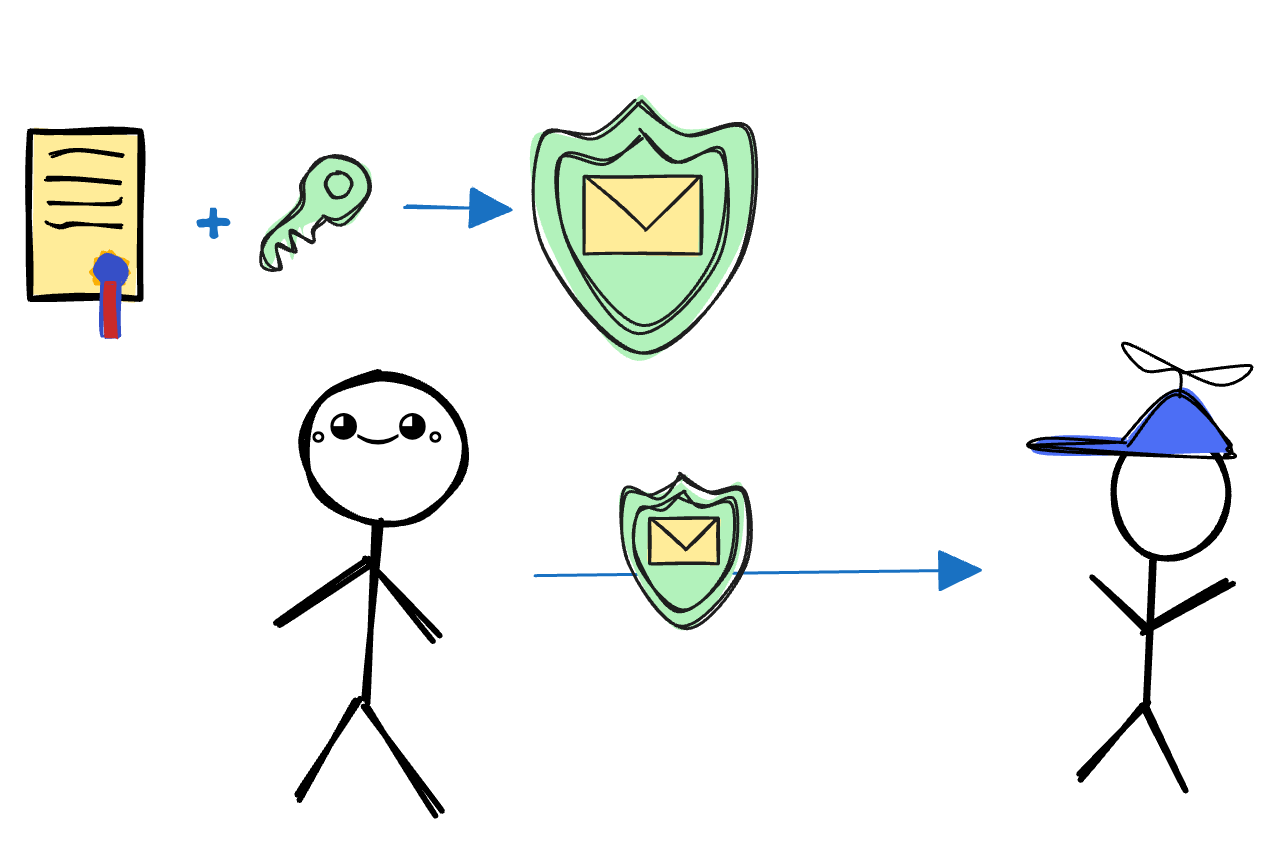
\includegraphics[width=0.5\textwidth]{images/lecture_5/CommitmentExample.png}
            \caption{Overview of a commitment scheme}
        \end{figure}
    \end{frame}

    \begin{frame}{Commitment Definition}
        \begin{definition}
            Commitment Scheme $\Pi_{\text{commitment}}$ is a tuple of three algorithms: $\Pi_{\text{commitment}} = (\mathsf{Setup}, \mathsf{Commit}, \mathsf{Verify})$.

            \begin{enumerate}

                \item Setup ($1^{\lambda}$): returns public parameter \textit{pp} for both comitter and verifier;

                \item  Commit ($\mathsf{pp}, m, r$): returns a commitment $c$ to the message $m$ using public parameters \textit{pp} and, optionally, a secret opening hit $r$;

                \item  Open ($\mathsf{pp}, c, m, r$): verifies the opening of the commitment to the message $m$ with an opening hit $r$. 
            \end{enumerate}
        \end{definition}

    \end{frame}

    \begin{frame}{Commitment Scheme Properties}
        \begin{definition}
            \begin{enumerate}
                \item \textit{Hiding: } verifier should not learn any additional information about the message given only the commitment $\mathcal{C}$.
                \begin{enumerate}
                    \item \textit{Perfect hiding}: adversary with any computation capability tries even forever cannot understand what you have hidden.
                    \item \textit{Computationally hiding}: we assume that the adversary have limited computational resources and cannot try forever to recover hidden value.
                \end{enumerate}
                
                \item \textit{Binding: } prover could not find another message $m_1$ and open the commitment $\mathcal{C}$ without revealing the commited message $m$.
                \begin{enumerate}
                    \item \textit{Perfect binding}: adversary with any computation capability tries even forever cannot find another $m_1$ that would result to the same $\mathcal{C}$.
                    \item \textit{Computationally binding}: we assume that the adversary have limited computational resources and cannot try forever.
                \end{enumerate}
            \end{enumerate}
        \end{definition}
        \begin{alertblock}{Note}
            Perfect hiding and perfect binding cannot be achived at the same time
        \end{alertblock}    
    \end{frame}

    \section{Hash-based Commitments}

    \begin{frame}{Hash-based commitments}

        As the name implies, we are using a cryptographic hash function \(H\) in such scheme.

        \begin{definition}
            \begin{enumerate}
                \item Prover selects a message $m$ from a message space $M$ which he wants to commit to:
                    $m \leftarrow \mathbb{M}$
            
                \item Prover samples random value $r$ from a challange space $C$ (usually called blinding factor) from $\mathbb{Z}$:
                    $r \xleftarrow{R} \mathbb{C}$
                
                \item Both values will be concatenated and hashed with the hash function $H$ to produce the commitment:
                    $\mathcal{C} = H(m \parallel r)$
            \end{enumerate}
        \end{definition}

    \end{frame}

    
	\begin{frame}{}
      \centering \Large
      \emph{Thanks for your attention!}
    \end{frame}
\end{document}